% +---------------------------------------------------------------------------+
% | english/chap/TheWayToWrite.tex                                            |
% |                                                                           |
% | Katakana or hiragana specific information                                 |
% |                                                                           |
% | Version: 0.1.1                                                            |
% |                                                                           |
% | Changes:                                                                  |
% |                                                                           |
% | 0.1.1 2023-06-05 Christian Külker <c@c8i.org>                             |
% |     - Improve English writing                                             |
% | 0.1.0 2022-09-10 Christian Külker <c@c8i.org>                             |
% |     - Initial version (disable input KanaPronunciation)                   |
% |                                                                           |
% +---------------------------------------------------------------------------+

\ifthenelse{\equal{hiragana}{\jtopic}}{%
\chapter{The Way to Write Hiragana}\jchap{平仮名の書き方}
% [o] LABEL
\label{chap:TheWayToWriteHiragana}
% [o] DESTINATIONS
% [o] INDEX
\ien{The Way to Write Hiragana}
\ien{hiragana!writing}
\ide{Hiragana!schreiben}
}{}%
\ifthenelse{\equal{katakana}{\jtopic}}{%
\chapter{The Way to Write Katakana}\jchap{片仮名の書き方}
% [o] LABEL
\label{chap:TheWayToWriteKatakana}
% [o] DESTINATIONS
% [o] INDEX
\ien{The Way to Write Katakana}
\ien{katakana!writing}
\ide{Katakana!schreiben}
}{}%
% [o] DESTINATIONS
\ifor{gojūonzu}{五十音図}{ごじゅうおんず}{50@50 Laute Tafel}
\ifor{mora}{モーラ}{もーら}{Mora}
\ifor{space character}{空白文字}{くうはく・もじ}{Leerzeichen}
\ifor{kanji}{漢字}{かんじ}{Kanji}

This chapter explains how to read and write \jkanavoc. After introducing the
sound structure, the traditional way of displaying and ordering \jtopic is
presented. A short section lists the functions of \jtopic, what \jtopic is used
for. The following section briefly introduces the pronunciation. Since this
book focuses on writing, the majority of the sections teach how to write
\jtopic and inform about special \jtopic as well as general punctuation. The
last part is about rarely used \jtopic.

\jscript{} derived from \textbf{Chinese} characters, called
\hyperref[sec:Kanji]{kanji}. All \jtopic{} together form a complete phonetic
script with less than 50 characters (or morae). This script can be used to
write all Japanese words.

\ifor{gojūonzu}{五十音図}{ごじゅうおんず}{50@50 Laute Tafel}

The \textbf{\jtopic} collection is usually displayed in the
\hyperref[sec:Gojuonzu]{gojūonzu} (lit. table of fifty sounds), a grid of 10x5
fields in which the characters are displayed. Although the
\hyperref[sec:Gojuonzu]{gojūonzu} nominally contains 50 characters, the grid is
not completely filled. There is also an extra character at the end. So with
five columns and one extra character, the current number of \textbf{\jtopic} is
47. %
\ifthenelse{\equal{hiragana}{\jtopic}}{
The script has no character for doubling a vowel (which would not be displayed
in the \hyperref[sec:Gojuonzu]{gojūonzu} anyway). Unlike \textbf{katakaka} with
47, \textbf{hiragana} has 46 different characters, still under 50.
}{}%
\ifthenelse{\equal{katakana}{\jtopic}}{
If we count the character for doubling a vowel (which is unfortunately not
shown in the \hyperref[sec:Gojuonzu]{gojūonzu}). Unlike \textbf{hiragana} with
46, \textbf{katakana} has 47 different characters, still under 50.
}{}%

\section{Gojūonzu}\jsec{五十音図}
% [o] LABEL
\label{sec:Gojuonzu}
% [o] INDEX DESTINATION (DEF)
\ifor{gojūonzu}{五十音図}{ごじゅうおんず}{50@50 Laute Tafel}
% [o] INDEX TARGET
\ifor{kana}{仮名}{かな}{Kana}
\ifor{iroha}{伊呂波}{いろは}{Iroha}

\newcommand{\lgojuonzu}{\ivoc{gojūonzu}{五十音図}{ごじゅうおんず}{Gojūonzu}}

Traditionally two ways exist to order Japanese \hyperref[sec:Kana]{kana}
characters. One of it is the \lgojuonzu{} (50 sound table), which is used more
often in modern times while the \hyperref[sec:Iroha]{iroha}\footnote{A poem
        with all \hyperref[sec:Kana]{kana} letters to remember easily. However
it is not standard Japanese anymore why it would be difficult to suggest to
learn.} was more popular in the older times.

The \textbf{gojuonzu} is a grid of 10 x 5 squares partly filled with
\hyperref[sec:Kana]{kana}, hiragana or katakana. The roman letters are not part
of the \textbf{gojuonzu} and are added for the convenience of the learner.

\section{Gojūonzu}\jsec{五十音図}
% [o] LABEL
\label{sec:Gojuonzu}
% [o] INDEX DESTINATION (DEF)
\ifor{gojūonzu}{五十音図}{ごじゅうおんず}{50@50 Laute Tafel}
% [o] INDEX TARGET
\ifor{kana}{仮名}{かな}{Kana}
\ifor{iroha}{伊呂波}{いろは}{Iroha}

\newcommand{\lgojuonzu}{\ivoc{gojūonzu}{五十音図}{ごじゅうおんず}{Gojūonzu}}

Traditionally two ways exist to order Japanese \hyperref[sec:Kana]{kana}
characters. One of it is the \lgojuonzu{} (50 sound table), which is used more
often in modern times while the \hyperref[sec:Iroha]{iroha}\footnote{A poem
        with all \hyperref[sec:Kana]{kana} letters to remember easily. However
it is not standard Japanese anymore why it would be difficult to suggest to
learn.} was more popular in the older times.

The \textbf{gojuonzu} is a grid of 10 x 5 squares partly filled with
\hyperref[sec:Kana]{kana}, hiragana or katakana. The roman letters are not part
of the \textbf{gojuonzu} and are added for the convenience of the learner.

\section{Gojūonzu}\jsec{五十音図}
% [o] LABEL
\label{sec:Gojuonzu}
% [o] INDEX DESTINATION (DEF)
\ifor{gojūonzu}{五十音図}{ごじゅうおんず}{50@50 Laute Tafel}
% [o] INDEX TARGET
\ifor{kana}{仮名}{かな}{Kana}
\ifor{iroha}{伊呂波}{いろは}{Iroha}

\newcommand{\lgojuonzu}{\ivoc{gojūonzu}{五十音図}{ごじゅうおんず}{Gojūonzu}}

Traditionally two ways exist to order Japanese \hyperref[sec:Kana]{kana}
characters. One of it is the \lgojuonzu{} (50 sound table), which is used more
often in modern times while the \hyperref[sec:Iroha]{iroha}\footnote{A poem
        with all \hyperref[sec:Kana]{kana} letters to remember easily. However
it is not standard Japanese anymore why it would be difficult to suggest to
learn.} was more popular in the older times.

The \textbf{gojuonzu} is a grid of 10 x 5 squares partly filled with
\hyperref[sec:Kana]{kana}, hiragana or katakana. The roman letters are not part
of the \textbf{gojuonzu} and are added for the convenience of the learner.

\input{../content/tab/\jtopic/Gojuonzu}

The later adopted /n/ was added as one square or in the above example as the
11th line. Even though there are less than 50 letters and more than 50 squares
out of historical reason the name used is still \textbf{gojuonzu}.

For more explanations please read the chapter
\nameref{chap:TheWayToWriteKatakana} and look at the various examples of the
\textbf{gojuonzu} in the appendix starting with \nameref{chap:KatakanaTables}
on page \pageref{chap:KatakanaTables} up to page
\pageref{sec:KatakanaMikachanPB}.



The later adopted /n/ was added as one square or in the above example as the
11th line. Even though there are less than 50 letters and more than 50 squares
out of historical reason the name used is still \textbf{gojuonzu}.

For more explanations please read the chapter
\nameref{chap:TheWayToWriteKatakana} and look at the various examples of the
\textbf{gojuonzu} in the appendix starting with \nameref{chap:KatakanaTables}
on page \pageref{chap:KatakanaTables} up to page
\pageref{sec:KatakanaMikachanPB}.



The later adopted /n/ was added as one square or in the above example as the
11th line. Even though there are less than 50 letters and more than 50 squares
out of historical reason the name used is still \textbf{gojuonzu}.

For more explanations please read the chapter
\nameref{chap:TheWayToWriteKatakana} and look at the various examples of the
\textbf{gojuonzu} in the appendix starting with \nameref{chap:KatakanaTables}
on page \pageref{chap:KatakanaTables} up to page
\pageref{sec:KatakanaMikachanPB}.



This document is structured according to the \hyperref[sec:Gojuonzu]{gojūonzu},
five \textbf{\jtopic} are introduced in one section to be learned together.

\ifor{space character}{空白文字}{くうはく・もじ}{Leerzeichen}
\ifor{homophone}{同音異語}{どうおん・いご}{Homophon}
\ija{同音語}

Although \textbf{\jtopic} can be used by itself to express the complete content
of the Japanese language, it is rarely used as such. The use of all Japanese
scripts \textbf{hiragana}, \textbf{katakana} and \hyperref[sec:Kanji]{kanji}
has the advantage that word boundaries can be easily seen and the
\hyperref[sec:SpaceCharacter]{space character} is unnecessary. So a Japanese
\textbf{\jtopic} sentence with only \textbf{\jtopic} and no
\hyperref[sec:SpaceCharacter]{space character} is hard to understand because it
is impossible to distinguish words. However, even if
\hyperref[sec:SpaceCharacter]{space character} were introduced as in Roman
languages, Japanese has so many \hyperref[sec:Homophone]{homophones} that it
would still be very difficult to impossible to understand sentences.
Especially \hyperref[sec:Kanji]{kanji} give context and meaning. Therefore, the
boundaries of script types (\hyperref[sec:Hiragana]{hiragana},
\hyperref[sec:Katakana]{katakana}, and \hyperref[sec:Kanji]{kanji}) are the
most important indicators of word boundaries.

\ifor{hiragana}{平仮名}{ひらがな}{Hiragana}
\ifor{katakana}{片仮名}{かたかな}{Katakana}
\ifor{okurigana}{送り仮名}{おくりがな}{Okurigana}
\ien{role}\ija{機能}\ija{きのう}\ide{Funktion}
\ide{Rolle}

\phantomsection
\label{sec:role}

In the Japanese written language, each character has a role. The role of
\textbf{\jtopic} has changed over time. The last big change was after the end
of World War II and \textbf{\jtopic} got the roles it still has today and they
are fixed for the time being.

\bigskip

% +---------------------------------------------------------------------------+
% | content/english/tab/Function.tex                                          |
% |                                                                           |
% | Table of hiragana and katakana functions                                  |
% |                                                                           |
% | Version: 0.1.0                                                            |
% |                                                                           |
% | Changes:                                                                  |
% |                                                                           |
% | 0.1.0 2022-09-10 Christian Külker <c@c8i.org>                             |
% |     - Initial release (moved from JapaneseWritingSystem.tex)              |
% |                                                                           |
% +---------------------------------------------------------------------------+
\ifthenelse{\equal{hiragana}{\jtopic}}{%
\begin{table}[h!]
\centering
\begin{tabular}{rp{15cm}}
 1. & Verb endings (furigana)\\
 2. & Adjective endings (furigana) \\
 3. & Words that have no kanji and are not written in katakana \\
 4. & Childrens books   \\
 5. & Educational material \\
 6. & Okurigana \\
 7. & Particles \\
 8. & \hyperref[sec:Manga]{Manga}\\
 9. & Words that have kanji, but the kanji is difficult to understand\\
10. & Onomatopoetica\\
11. & Transcription of kanji (for example in formulars, passports) \\
12. & Advertising might replace kanji or katakana for estetic reasons \\
13. & Sounds in the middle of a kanji word that are not covered by the kanji\\
14. & Honoric prefixes\\
15. & When one would like to be considered childish\\
16. & Some personal names (especially female) to make them cute \\

\end{tabular}
\caption{List of hiragana roles and functions}
\label{table:HiraganaFunction}
\end{table}
}{}

\ifthenelse{\equal{katakana}{\jtopic}}{%
\begin{table}[h!]
\centering
\begin{tabular}{rp{15cm}}
 1. & writing words of foreign origin\\
 2. & words that need to be emphasized\\
 3. & often indicate on-yomi in dictionaries\\
 4. & names of minerals \\
 5. & geological names \\
 6. & names of fauna (animals)\\
 7. & names of flora (plants)\\
 8. & partly onomatopoeias in \hyperref[sec:Manga]{manga}\\
 9. & sounds, like animal sounds or sounds made by humans\\
10. & telegrams (before 1988)\\
11. & banking system account names\\
12. & In literature (eg. \hyperref[sec:Manga]{manga}) words being spoken in a
(foreign) accent or "robotic" speech\\
13. & sometimes used as Furigana\\
14. & uncommon \hyperref[sec:Kanji]{Kanji}, eg. {皮膚科} {【ひふか】}
"dermatologist" written as {皮フ科}\\
15. & computer output (in 80s, before introduction of multi byte characters)\\
16. &some personal names (especially female) (common in the past: eg.
セツ (setsu))\\

\end{tabular}
\caption{List of katakana roles and functions}
\label{table:KatakanaFunction}
\end{table}
}{}


\medskip

\ifor{manga}{漫画}{まんが}{Manga}

Therefore, in commercials, \hyperref[sec:Manga]{manga} and literature
describing foreign concepts, \textbf{katakana} has a over proportionate use.

%% ---------------------------------------------------------------------------
\section{Pronunciation and Intonation}\jsec{発音とイントネーション}
% [o] LABEL
\label{sec:PronunciationAndIntonation}
\label{sec:Pronuciation}
\label{sec:Intonation}
% [o] INDEX
\ifor{pronuciation}{発音}{はつおん}{Aussprache}
\ifor{intonation}{イントネーション}{いんとねーしょん}{Betonung}
\ifor{Katakana}{片仮名}{かたかな}{Katakana}
\ifor{Hiragana}{平仮名}{ひらがな}{Hiragana}
\ifor{mora}{モーラ}{もーら}{Mora}
\ifor{Gojūonzu}{五十音図}{ごじゅうおんず}{50@50 Laute Tafel}

The \textit{pronunciation} of \hyperref[sec:Katakana]{Katakana} is the same as
for \hyperref[sec:Hiragana]{Hiragana}. Therefore every
\hyperref[sec:Syllable]{syllable}, more precise every \hyperref[sec:Mora]{mora}
corresponds to a \hyperref[sec:Katakana]{Katakana} character and is constructed
as 'consonant' + 'vowel' with the exception of |n|. This system of letter for
each \hyperref[sec:Mora]{mora} makes \textit{pronunciation} absolutely clear
with no ambiguities.  However the simplicity of
\hyperref[sec:Katakana]{Katakana} does not mean that \textit{pronunciation} in
Japanese is simple for English speakers as it is for Germans.  The rigid
structure of the fixed \hyperref[sec:Mora]{mora} sound in Japanese creates the
challenge of learning the proper intonation and duration of Japanese
\textit{pronunciation}.

Almost each Japanese word can be chunked into \hyperref[sec:Mora]{morae} of
high and low pitch witch is a crucial aspect of the spoken language. Compared
to Chinese, Japanese luckily have only two pitches: hi and low. Sometimes this
difference can be even important for the lexis. Homophones can have for example
a difference in pitch which make them distinguishable.  The intonation of high
and low pitches is a crucial aspect of the spoken language. One of the biggest
problems for obtaining a natural sounding \textit{pronunciation} is the
incorrect intonation. Many European or American learners speak without paying
attention to the correct pitch. That makes the speech sound non-natural for
Japanese. In some language course try to let the learner memorize the natural
pitch of a word or even teach rules for memorization. While there is clearly a
possibility for linguistic rules, they are hard to remember and master.
It is still possible to learn the correct
intonation by resorting to language learning techniques used by infants or
small children: mimicking native Japanese speakers. Therefore it is highly
advised to expose oneself to as many Japanese spoken language as possible and
to mimic it. Radio, podcasts, drama and television to name a few. However, it
is not advised to listen too much artificial sources like anime or commercials.

\bigskip
\begin{tabular}{rl}
-&every (yes \textbf{every}) \hyperref[sec:Mora]{mora} is \textit{pronounced} 
  with the same length\\
-&there is no short and long \hyperref[sec:Mora]{mora} or letters\\
-&every \hyperref[sec:Mora]{mora} has a pitch: high or low\\
-&every pitch matters\\
-&the pitch can change  sometimes with its context\\
-&the pitch can change with a dialect - however standard Japanese has well 
  defined pitches\\
\end{tabular}

\bigskip

The \textit{pronunciation} of \hyperref[sec:Katakana]{Katakana} is exactly the
same as for \hyperref[sec:Hiragana]{Hiragana} and most sounds are very close to
the Latin \textit{pronunciation} but in general are \textit{pronounced} a
little shorter without any stress. Only the /ra/ sounds, like in /ra/, /ri/,
/ru/, /re/ and /ro/ have no similarity in European languages. 


The sound of the Japanese /r/ is  neither a central nor a lateral flap, but may
vary between the two. To an English speaker, its pronunciation varies between a
flapped 'd' (as in American English buddy) and a flapped 'l'.
\href{http://en.wikipedia.org/wiki/Japanese_phonology}{(Wikipedia Japanese
Phonology)}.


The following table displays the \textit{pronunciation} in the
\hyperref[sec:Gojuonzu]{Gojūonzu}.

\ien{Rōmaji Gojūonzu}
\ien{Rōmaji}
\ien{Gojūon}
\ija{ローマ字五十音図}
\ija{ローマ字}
\bigskip
\begin{center}
%\LARGE
%\Huge
\Padding
\begin{tabular}{c||c|c|c|c|c|}
&\textbf{a}&\textbf{i}&\textbf{u}&\textbf{e}&\textbf{o}\\\hline\hline
\textbf{-}&a&i&u&e&o\\\hline
\textbf{k}&ka&ki&ku&ke&ko\\\hline
\textbf{s}&sa&shi&su&se&so\\\hline
\textbf{t}&ta&chi&tsu&te&to\\\hline
\textbf{n}&na&ni&nu&ne&no\\\hline
\textbf{h}&ha&hi&fu&he&ho\\\hline
\textbf{m}&ma&mi&mu&me&mo\\\hline
\textbf{y}&ya&&yu&&yo\\\hline
\textbf{r}&ra&ri&ru&re&ro\\\hline
\textbf{w}&wa&&&&o\\\hline
\textbf{{*}}&n&&&&\\\hline
\end{tabular}
\end{center}





% ---------------------------------------------------------------------------
\section{Writing Katakana Letters}\jsec{片仮名を一つづつ書く}
% [o] LABEL
\label{sec:WritingKatakanaLetters}
% [o] INDEX
% DESTINATION (DEF)
\ifor{Katakana}{片仮名}{かたかな}{Katakana} % TARGET

Writing \textit{Katakana words} start with writing single \textit{Katakana
letters}. Knowing the writing and reading of \textit{Katakana letters} is
essential to pronounce foreign words in Japanese correctly. And that is even
more important for learners who have good English knowledge, because it is very
tempting to pronounce English words in Japanese with original English
pronunciation, which is seldom understood\footnote{The reader might try to
order a cheeseburger at a fast food restaurant insted of a /chiizubaagaa/
(チーズバーガー).} by Japanese people who are used to their Japanese-English
pronunciation.

By learning \textit{Katakana} the understanding of morae and syllables will
also help to improve the pronunciation and understanding of Japanese.

\textit{Katakana} as most letters are a joint combination of strokes. For the
writing of \textit{Katakana} some rules are important, which are presented here
out of order.


\begin{description}

\item[Order:] The order of strokes is important. In section
\ref{sec:StrokeOrderMatter} on page \pageref{sec:StrokeOrderMatter} more can be
found.

\item[Fasted Method of Writing:] Often the fastest possible method of writing
or order of strokes is the correct one.  Often from left upper corner to right
lower corner. But exceptions do exist.

\item[The characters (letters) are \textit{not} symmetric.]

\item[All characters (letters) occupy a square.]

\item[The aesthetic:] What make the character to a beautiful character? The
answer is different for each character.

Following some possibilities of rule generation for the character ``u''
 {「ウ」 }:

\bigskip \CharacterExplanation{u-guide2}{The most important feature is that the
second and third line do not align. This is not an accident.}

\bigskip \CharacterExplanation{u-guide0}{Except many
\hyperref[sec:Hiragana]{Hiragana} for some \textit{Katakana} the base line is
aligned with horizon. As with this character. }


\bigskip \CharacterExplanation{u-guide1}{Also the start (or turning) points of
all other lines are aligned vertically. Which gives this \textit{Katakana} its
unique square look.}


\bigskip \CharacterExplanation{u-guide}{All together some lines need to be
remembered to write the letter beautiful.}

\bigskip

\item[A different logic:] A little bit less the
\hyperref[sec:Hiragana]{Hiragana}, but also in \textit{Katakana} there are some
lines that do not align horizontally  or vertically. Or to say it differently
some characters are not straight on purpose.

\end{description}

On top of this the following is most likely valid: only if one can write a
letter it is (easier) possible to learn faster and memorize it.


%----------------------------------------------------------------------------
\subsection{Stroke Order Matter!}\jsubsec{書き順事項}
% [o[ LABEL
\label{sec:StrokeOrderMatter}
% [o] INDEX

Some European individualists might ask themselves \textit{"Why do I have to
remember the order of strokes - I don't obay this in my language - and who
defined this in the first place (if not me)?"} and this seems obvious in
Europe. However some reason for order exist.

% 書き順事項 【かきじゅんじこう】

\begin{description}

\item[1. Impression:] it makes an unprofessional impression to Japanese, if one
writes characters in the wrong order. Some laughs can be observed at least.

\item[2. Tests:]  in some tests/exams (in Japan) the order of strokes will be
tested and one gets 0 points for the wrong order.

\item[3. Time Savings:] In the most cases the predefined order is the fastest
way to write a character. Overall once save (life) time.

\item[4. Readability:] in some cases characters become readable only (or
beautiful) if the order is correct.

\item[5. Confusion Danger:] for some characters, the order is utmost
important. If not obeyed it is very likely (ie, almost certain) that these
characters become a candidate for wrong interpretation.

\end{description}
\normalsize

\newpage
%----------------------------------------------------------------------------
\subsection{Example /u/ }\jsubsec{{「ウ」の例} }
% [o] LABEL
\label{subsec:ExampleU}
% [o] INDEX

The \textit{Katakana} /u/ is written as {「ウ」} in Japanese. The character is
composed out of the following three components:

\bigskip
\CharacterExplanation{uds1}{This is stroke 1}
\bigskip
\CharacterExplanation{uds2}{This is stroke 2}
\bigskip
\CharacterExplanation{uds3}{This is stroke 3}

Of course the strokes need to be at the right place. So better always think or
draw a frame aound. Or even better write the strokes into a frame from the
beginning!

\bigskip
\CharacterExplanation{udss1}{This is stroke 1 in a square frame}
\bigskip
\CharacterExplanation{udss2}{This is stroke 2 in a square frame}
\bigskip
\CharacterExplanation{udss3}{This is stroke 3 in a square frame}


%\begin{center}
%\textbf{Stroke 1:} 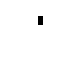
\includegraphics[trim= 00 15 00 00]{../share/katakana/uds1.pdf}
%\textbf{Stroke 2:} 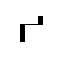
\includegraphics[trim= 00 15 00 00]{../share/katakana/uds2.pdf}
%\textbf{Stroke 3:} 
\includegraphics[trim= 00 15 00 00]{../share/katakana/uds3.pdf}
%\end{center}
\bigskip

This components have to be written in the above mentioned enumeration order one
after another. (The first example is without frame)

\bigskip
\CharacterExplanation{udg1}{This is stroke 1 in context}
\bigskip
\CharacterExplanation{udg2}{This is stroke 2 in context}
\bigskip
\CharacterExplanation{udg3}{This is stroke 3 in context}

%\begin{center}
%\textbf{Stroke 1:} 
\includegraphics[trim= 00 15 00 00]{../share/katakana/udg1.pdf}
%
%\textbf{Stroke 2:} 
\includegraphics[trim= 00 15 00 00]{../share/katakana/udg2.pdf}
%
%\textbf{Stroke 3:} 
\includegraphics[trim= 00 15 00 00]{../share/katakana/udg3.pdf}
%\end{center}

\bigskip
\CharacterExplanation{udgs1}{This is stroke 1 in context in a square frame}
\bigskip
\CharacterExplanation{udgs2}{This is stroke 2 in context in a square frame}
\bigskip
\CharacterExplanation{udgs3}{This is stroke 3 in context in a square frame}

\bigskip

In the \textit{Katakana} training section in this document the order will be
introduced as red numbers and arrows which give the approximate direction where
to place the writing device.

%\begin{center}
% 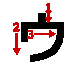
\includegraphics[trim= 00 05 00 00]{../share/katakana/us.pdf}
%\end{center}
\bigskip

\CharacterExplanation{us}{Write the first short stroke straight from up to
down. Then - and this is difficult, place the second stroke in the correct
distance from the first one. Luckily this is also a straight stroke from up to
down. }

\bigskip

Of course the perception changes if the character is written in a square.
Remember that it is better to write the character in a square, because the
correct spaces between the character and the frame also determinates its
beauty.

\bigskip

\CharacterExplanation{uss}{The first stroke in the frame is not difficult, as
mentioned before it goes from straight up to down. However the frame helps because now
we understood that it is centered. The second stroke becomes also easier in a
frame because it is written at the edge of the character. After some time and
experience this is better understood. The last stroke has to join the first and
second stroke. That is still difficult with or without a frame.}

\bigskip

%----------------------------------------------------------------------------
\subsection{Stroke Types}\jsubsec{筆画の種類}
% [o] LABEL
\label{sec:StrokeTypes}
\label{sec:Stroke}
\label{subsec:StrokeTypes}
% [o] INDEX
\ifor{stroke types}{筆画の種類}{ひっかくのしゅるい}{Strich Typen}
\ifor{stroke}{筆画}{ひっかく}{Strich}
\ifor{Hiragana}{平仮名}{ひらがな}{Hiragana}
\ifor{Kanji}{漢字}{かんじ}{Kanji}

In European language there is no idea to have different \textit{stroke} types
unless one enter the field of calligraphy. In Japanese there are different kind
of \textit{strokes}.  Most important for \hyperref[sec:Kanji]{Kanji}, second
important for \hyperref[sec:Hiragana]{Hiragana} and least important for
\textit{Katakana} since \textit{Katakana} is also used for a bold replacement.
Due to this fact the five different type of Japanese \textit{strokes}
({筆画の種類} {【ひっかくのしゅるい】}) will not repeated here. For now it is
perfectly fine to make all \textit{strokes} equally thick.



%\input{../share/sec/WritingKatakanaSentences}
% +---------------------------------------------------------------------------+
% | SpecialKanaCharacters.tex                                                 |
% |                                                                           |
% | Collect special hiragana and katakana characters                          |
% |                                                                           |
% | Version: 0.1.0                                                            |
% |                                                                           |
% | Changes:                                                                  |
% |                                                                           |
% | 0.1.0 2022-08-02 Christian Külker <c@c8i.org>                             |
% |     - Merge katakana and hiragana                                         |
% |                                                                           |
% +---------------------------------------------------------------------------+

\ifthenelse{\equal{hiragana}{\jtopic}}{%
\section{Special Hiragana Characters}\jsec{特別ひらがな}
% LABEL
\label{sec:SpecialHiraganaCharacters}
\label{sec:SpecialKanaCharacters}
% INDEX
\ifor{special hiragana characters}{特別ひらがな}{とくべつひらがな}{Spezielle Hiragana Zeichen}
}{}
\ifthenelse{\equal{katakana}{\jtopic}}{%
\section{Special Katakana Characters}\jsec{特別カタカナ}
% LABEL
\label{sec:SpecialKatakanaCharacters}
\label{sec:SpecialKanaCharacters}
% INDEX
\ifor{special katakana characters}{特別カタカナ}{とくべつかたかな}{Spezielle Katakana Zeichen}
}{}
% INDEX
\ifor{hiragana}{平仮名}{ひらがな}{Hiragana}
\ifor{gojūonzu}{五十音図}{ごじゅうおんず}{50@50 Laute Tafel}

As mentioned before both \textbf{kana} syllables are almost the same, except
the shape. This is especcially true for the \hyperref[sec:Gojuonzu]{gojūonzu
(50 sound table)}. This section will show the special characters, some are
different from the ordninary \jtopic{} set.

%TODO check if point changes orientation and alignment in case of changing
%writing direction.

\ifthenelse{\equal{hiragana}{\jtopic}}{%
\subsection{Doubling Vowels in Hiragana}\jsubsec{ひらがなでの倍増母音}
}{}
\ifthenelse{\equal{katakana}{\jtopic}}{%
\subsection{Doubling Vowels in Katakana}\jsubsec{カタカナでの倍増母音}
}{}
% [o] LABEL
\label{subsec:DoublingVowelsIn\jscript}
\label{subsec:DoublingVowels}
\label{sec:DoublingVowelsIn\jscript}
\label{sec:DoublingVowels}
% [o] INDEX
\ifor{doubling vowels}{倍増母音}{ばいぞうぼいん}{Vokalverdopplung}
\ifor{repetition mark}{繰り返し記号}{くりかえしきごう}{Wiederholungszeichen}
\ifor{hiragana}{平仮名}{ひらがな}{Hiragana}
\ifor{katakana}{片仮名}{かたかな}{Katakana}

% ひらがなでの倍増母音 【ばいぞうぼいん】
% カタカナでの倍増母音 【ばいぞうぼいん】


\ifthenelse{\equal{hiragana}{\jtopic}}{%

The usual way to double a vowl in \textbf{hiragana} is to write that hiragana
again. In the hiragana \jquotesingleja{お} character can be doubled with either
\jquotesingleja{お} or \jquotesingleja{お} . So \jtl{ō} becomes either
\jquotesingleja{おお} or \jquotesingleja{おう}. There is no rule to it. This
has to be rememberd. However in most cases \jquotesingleja{お} is doubled as
\jquotesingleja{おお}.

}{}
\ifthenelse{\equal{katakana}{\jtopic}}{%

Special \hyperref[sec:Katakana]{katakana} characters do also exists. The most
important character is \ivoc{chōon}{長音}{ちょうおん}{Chōon} the plain
iteration character \jquotesingleja{ー}, written as a stroke. It is one of the
very few which changes orientation according the writing orientation. When
writing katakana from left to right the iteration character is horizontal,
while writing katakana from up to down it is vertical. The function of this
character is to double the previous mora.  This is also different from
\hyperref[sec:Hiragana]{hiragana}. (For doubling als other katakana caracter,
refere to section \nameref{sec:Iteration} on page \pageref{sec:Iteration}.)

\bigskip

\CharacterExplanation{k-iteration-s}{In standard gothic fonts the
\hyperref[sec:Katakana]{katakana} iteration character is just a straight line
and it is not possible to understand in which direction it has to written. }

\bigskip

\CharacterExplanation{k-iteration-sm}{However if it is written with a different
font or with a brush it is clearly visible that in horizontal writing it is
written from left to right.}

}{}
\bigskip

%\definecolor{orange}{rgb}{1,0.5,0}
%\definecolor{mygreen}{rgb}{.2,1,.2}

\setCJKfamilyfont{cjk-horiz-m}[Script=CJK,RawFeature=horizontal]{IPAMincho}
\setCJKfamilyfont{cjk-horiz-g}[Script=CJK,RawFeature=horizontal]{IPAPGothic}
%\setCJKfamilyfont{cjk-vert}[Script=CJK,RawFeature=vertical]{Kozuka Gothic Pro M}
\setCJKfamilyfont{cjk-vert-m}[Script=CJK,RawFeature=vertical]{IPAMincho}
\setCJKfamilyfont{cjk-vert-g}[Script=CJK,RawFeature=vertical]{IPAPGothic}

\bigskip
\textit{Example:}

\bigskip

\begin{figure}[H]
\begin{center}
\begin{tabular}{p{7cm}p{7cm}}
Katakana:&Hiragana:\\
\CJKfamily{cjk-horiz-h}
\Huge カ\textbf{\color{magenta}ー}ド \jtl{kaado} &
\Huge か\textbf{\color{magenta}あ}ど \jtl{kaado}\\
\CJKfamily{cjk-horiz-g}
\Huge カ\textbf{\color{magenta}ー}ド \jtl{kaado} &
                                                \\
\end{tabular}
\end{center}
\caption{Kana vowl doubling example}
\label{fig:KanaVowlDoublingExample}
\end{figure}

\bigskip

This character is very often used and makes \hyperref[sec:Hiragana]{hiragana}
for this easier then hiragana. The long vowel ambiguity do not exist.

As mentioned above the orientation of the \hyperref[sec:Katakana]{katakana}
iteration character changes with the direction of writing. The above example
with different writing orientation.

\medskip
\textit{Example:}

\medskip


\begin{figure}[H]
\begin{center}
\begin{tabular}{p{3.5cm}p{3.5cm}p{3.5cm}m{3.5cm}}
horizontally&
\mbox{
\begin{minipage}{3.2cm}
\CJKfamily{cjk-horiz-h}
\Huge カ\textbf{\color{magenta}ー}ド
\CJKfamily{cjk-horiz-g}
\Huge カ\textbf{\color{magenta}ー}ド
\end{minipage}
}
& vertically &
\raisebox{-.5\height}{
\mbox{
\rotatebox{-90}{
\begin{minipage}{3.2cm}
\CJKfamily{cjk-vert-m}
\Huge カ\textbf{\color{magenta}ー}ド
\CJKfamily{cjk-vert-g}
\Huge カ\textbf{\color{magenta}ー}ド
\end{minipage}
}
}
}
\\
\end{tabular}
\end{center}
\caption{Katakana horizontal and vertical vowl doubling example}
\label{fig:KatakanaHirzontalVerticalVowlDoublingExample}
\end{figure}

\medskip

% めったに使われない片仮名 【めったにつかわれないかたかな】
\ifthenelse{\equal{hiragana}{\jtopic}}{%
    \subsection{Seldom Used Hiragana}\jsubsec{めったに使われない平仮名}\label{subsec:SeldomlyUsedHiragana}

\ifor{voice!new writing}{声}{こえ}{Stimme!neue Schreibweise}
\ifor{voice!old writing}{声}{こゑ}{Stimme!alte Schreibweise}

All \textbf{hiragana} mentioned in the \hyperref[sec:Gojuonzu]{gojūonzu (50
sound table)} are used. There is no obsolete character in the table unlike the
\textbf{katakana} \jtl{wo} \jquotesingleja{ヲ}. However sometimes one can find
a \textbf{gojūonzu} with the additional chrarcters: \jquotesingleja{ゐ} wi,
pronounced as \jtl{i}, and \jquotesingleja{ゑ} we, pronounced \jtl{e}, in the
\jtl{wa} row. This characters are old characters and normally not used. It is
safe to skip learning this characters.  Words that used to have
\jquotesingleja{ゐ} had it replaced with \jquotesingleja{い} \jtl{i} and words
that used to have \jquotesingleja{ゑ} had it replaced with \jquotesingleja{え}
\jtl{e}. Examples: old \jquotesingleja{ゐる} is now written
\jquotesingleja{いる} \jtl{iru} ({居る} - to be somewhere), old
\jquotesingleja{こゑ} is now written as \jquotesingleja{こえ} \jtl{koe} ({声} -
voice).

}{}
% めったに使われない平仮名 【めったにつかわれないひらがな】
\ifthenelse{\equal{katakana}{\jtopic}}{%
    \subsection{Seldom Used Katakana}\jsubsec{めったに使われない片仮名}\label{subsec:SeldomlyUsedKatakana}

Since all particles are written in \textbf{hiragana} the particle \textit{wo},
pronounced as \jtl{o}, is written with the hiragana \jquotesingleja{を}. The
equivalent \textbf{katakana} wo \jquotesingleja{ヲ}, also pronounced \jtl{o},
is part of the \hyperref[sec:Gojuonzu]{gojūonzu}, however it is not used in
modern texts and it is not a particle. It was used in old texts (like
telegrams). Therefore the katakana \jquotesingleja{ヲ} can be skipped to learn.

\label{sec:Wi}
\label{sec:We}
\ifor{we}{ヱ}{エ}{we}
\ifor{wi}{ヰ}{イ}{wi}

In some cases the \textbf{gojūonzu} contain additional chrarcters:
\jquotesingleja{ヰ} wi, pronounced as \jtl{i}, and \jquotesingleja{ヱ} we,
pronounced \jtl{e}, in the \jtl{wa} row. This characters are old characters and
normally not used. It is safe to skip learning this characters. Words that used
to have \jquotesingleja{ヰ} had it replaced with \jquotesingleja{イ} \jtl{i}
and words that used to have \jquotesingleja{ヱ} had it replaced with
\jquotesingleja{エ} \jtl{e}.

}{}





